On this part we outline the clustering techniques used for the metrics grouping, the heuristic to do an automated classification mechanisms and finally the association rule used to find the metric which impacted on the performance of the executions.\\

% \textbf{Clustering techniques}
% \textit{ Supervised and non-supervised machine learn methods}\\
%     Supervised learning is the machine learning task of inferring a function from labeled training data. The training data consist of a set of training examples. In supervised learning, each example is a pair consisting of an input object (typically a vector) and a desired output value (also called the supervisory signal). A supervised learning algorithm analyzes the training data and produces an inferred function, which can be used for mapping new examples. 
    
%     Unsupervised machine learning is the machine learning task of inferring a function to describe hidden structure from "unlabeled" data (a classification or categorization is not included in the observations). Since the examples given to the learner are unlabeled, there is no objective evaluation of the accuracy of the structure that is output by the relevant algorithm—which is one way of distinguishing unsupervised learning from supervised learning and reinforcement learning.
    
\textit{Support Vector Machines}\\
In machine learning, support vector machines are supervised learning models with associated learning algorithms that analyze data used for classification and regression analysis. Given a set of training examples, each marked as belonging to one or the other of two categories, an SVM training algorithm builds a model that assigns new examples to one category or the other, making it a non-probabilistic binary linear classifier. 
Besides teaching the model, the restriction is another drawback of using SVMs. The major drawback of this model is the division in two groups, so relevant information could be lost and no further comparison technique could be applied later.

    
% \textit{Mean Swift}\\
%     MeanShift clustering aims to discover blobs in a smooth density of samples. It is a centroid based algorithm, which works by updating candidates for centroids to be the mean of the points within a given region. These candidates are then filtered in a post-processing stage to eliminate near-duplicates to form the final set of centroids.
%     Given a candidate centroid x i for iteration t, the candidate is updated according to the following equation:
    
%     %x_i^{t+1} = x_i^t + m(x_i^t)
    
%     Where N(xi) is the neighborhood of samples within a given distance around xi and m is the mean shift vector that is computed for each centroid that points towards a region of the maximum increase in the density of points. This is computed using the following equation, effectively updating a centroid to be the mean of the samples within its neighborhood:
%     %m(x_i) = \frac{\sum_{x_j \in N(x_i)}K(x_j - x_i)x_j}{\sum_{x_j \in N(x_i)}K(x_j - x_i)}
    
%     The algorithm automatically sets the number of clusters, instead of relying on a parameter bandwidth, which dictates the size of the region to search through. This parameter can be set manually, but can be estimated using the provided estimate bandwidth function, which is called if the bandwidth is not set.
%     The algorithm is not highly scalable, as it requires multiple nearest neighbor searches during the execution of the algorithm. The algorithm is guaranteed to converge, however the algorithm will stop iterating when the change in centroids is small \cite{mean_swift}.

\textit{Percentage classification}\\
The percentage classification was done by comparing the metrics and separate them by a percentage threshold, which is the mean of the group. The percentage classification is interesting considering sometimes that the distribution is not so spaced to create clusters. The naive classification will draw a group even when they are too close and would be in just one group for other clustering techniques.
    
\textit{K-means}\\
K-means is a simple unsupervised machine learning algorithm that groups a dataset into a user-specified number (k) of clusters. The algorithm is somewhat naive it clusters the data into k clusters, even if k is not the right number of clusters to use. Therefore, when using k-means clustering, users need some way to determine whether they are using the right number of clusters.
Since, the number of groups must be known before applying the k-means, another technique needs to be applied in order to find the appropriate number of groups (k). A similar algorithm, but ofr one 1D is called Jenks Natural Breaks \cite{break}.
    
     
    
\textit{Comparing Models}\\
Comparing the three techniques described above, the conclusions were. First, the SVM model was able to delimit the difference between the slow executions and fast executions. However, the delimitation is in just two groups. \\
The second mechanism, Percentage classification, is a unsupervised mechanism and leads to segregation of data even if they are homogeneously distributed among the dataset. \\
Finally the k-means algorithm is efficient but requires the number of groups to be used in the classification process. Comparing the models we developed the technique to use an heuristic classification to make the clustering process automatic.
    
    
\textit{Auto Clustering}\\
Considering the models shown above, we chose to develop a non-supervised method, called auto clustering. The possibility to use an automated approach is more interesting for us in comparison with a non-automated methods, mainly because we aim not to use the data to train the model. Therefore we implemented a version of comparative k-means using the SSE (sum of square errors) variability information, plus an heuristic evaluation. This technique can be used for an arbitrary dimension of since the amount of difference, SSE (sum of squared error), can be calculated on those cases \cite{multi_dimentionals_sse}.
    
\subsection{Automatic Clustering through heuristic Evaluation}

    \textit{Elbow method}\\
    One method to quantitatively measure the number of clusters is the elbow method. This method compares the sum of squared errors (SSE) considering several numbers of groups from the classification used. 
    The elbow method gives the possibility to use the SSE to find the elbow value, which can be defined as a value which the SSE changes its behaviour abruptly. In our cases, the elbow value is when the SSE stop decreasing substantially.
    
    However, the elbow method does not guarantee a perfect match in cases which the data is well distributed. Instead, the analysis of the SSE can give a smooth curve and the best value for number of groups is not precisely defined. In cases like this, we developed another clustering based on the mean distance of the data.
    %try a different method for determining the optimal k, such as computing silhouette scores, or we might reevaluate whether clustering is the right thing to do on our data.
    
    \textit{Heuristic Evaluation}\\
    To compare the SSE values, we needed also to do an heuristic function which compares the different values of the SSE to compute the Elbow. 
    Therefore, we use this approach to compare several runs of classifications and extract the one with less squared errors. The used heuristic is to take as optimal group the biggest gap on an array of SSE values. 
    
    The Figure \ref{fig:sse}, shows an illustration of the SSE and the elbow value. The elbow value is the number that marks the change on the path of the function, in our case the number of groups is 2. 
     \begin{figure}[h]
     \vspace{-10pt}
      \centering
        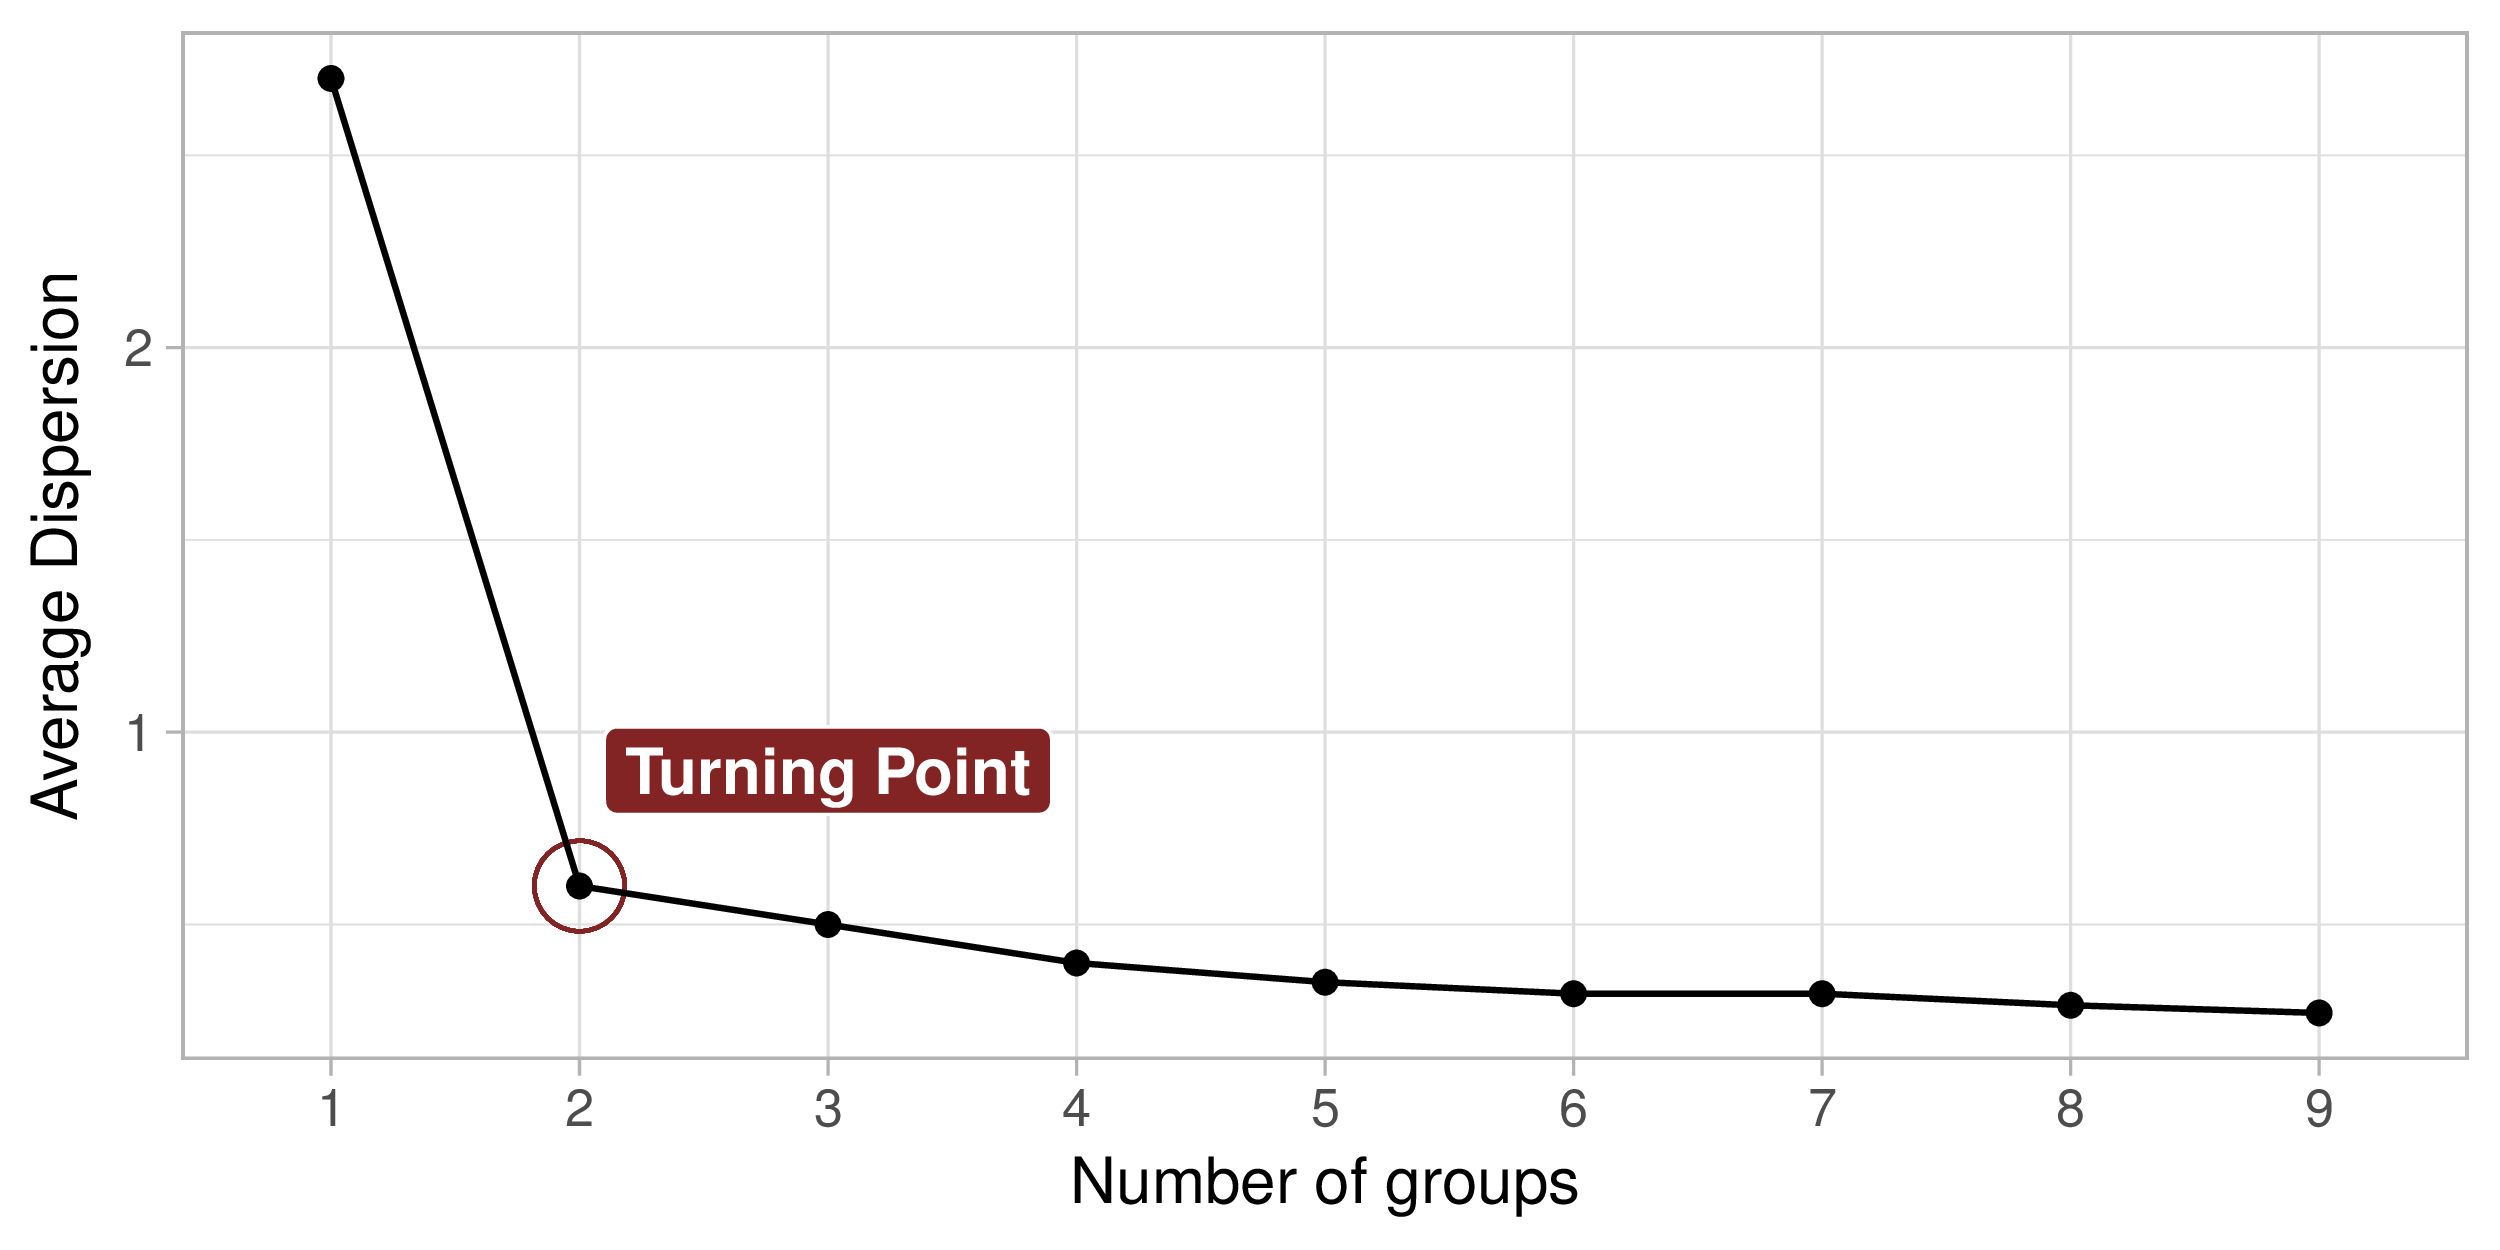
\includegraphics[width=0.50\textwidth]{figures/sse-groups.png}
        \caption{Elbow method: SSE Comparison}
        \label{fig:sse}
        \vspace{-10pt}
    \end{figure}
    
    The Figure \ref{fig:grouping-hist}, shows the SSE differences considering several number of groups. This image clearly shows the biggest gap between one and two groups, but since we are assuming that the data has gaps, we are not using one as the optimal number.
    
    \begin{figure}[h]
      \centering
        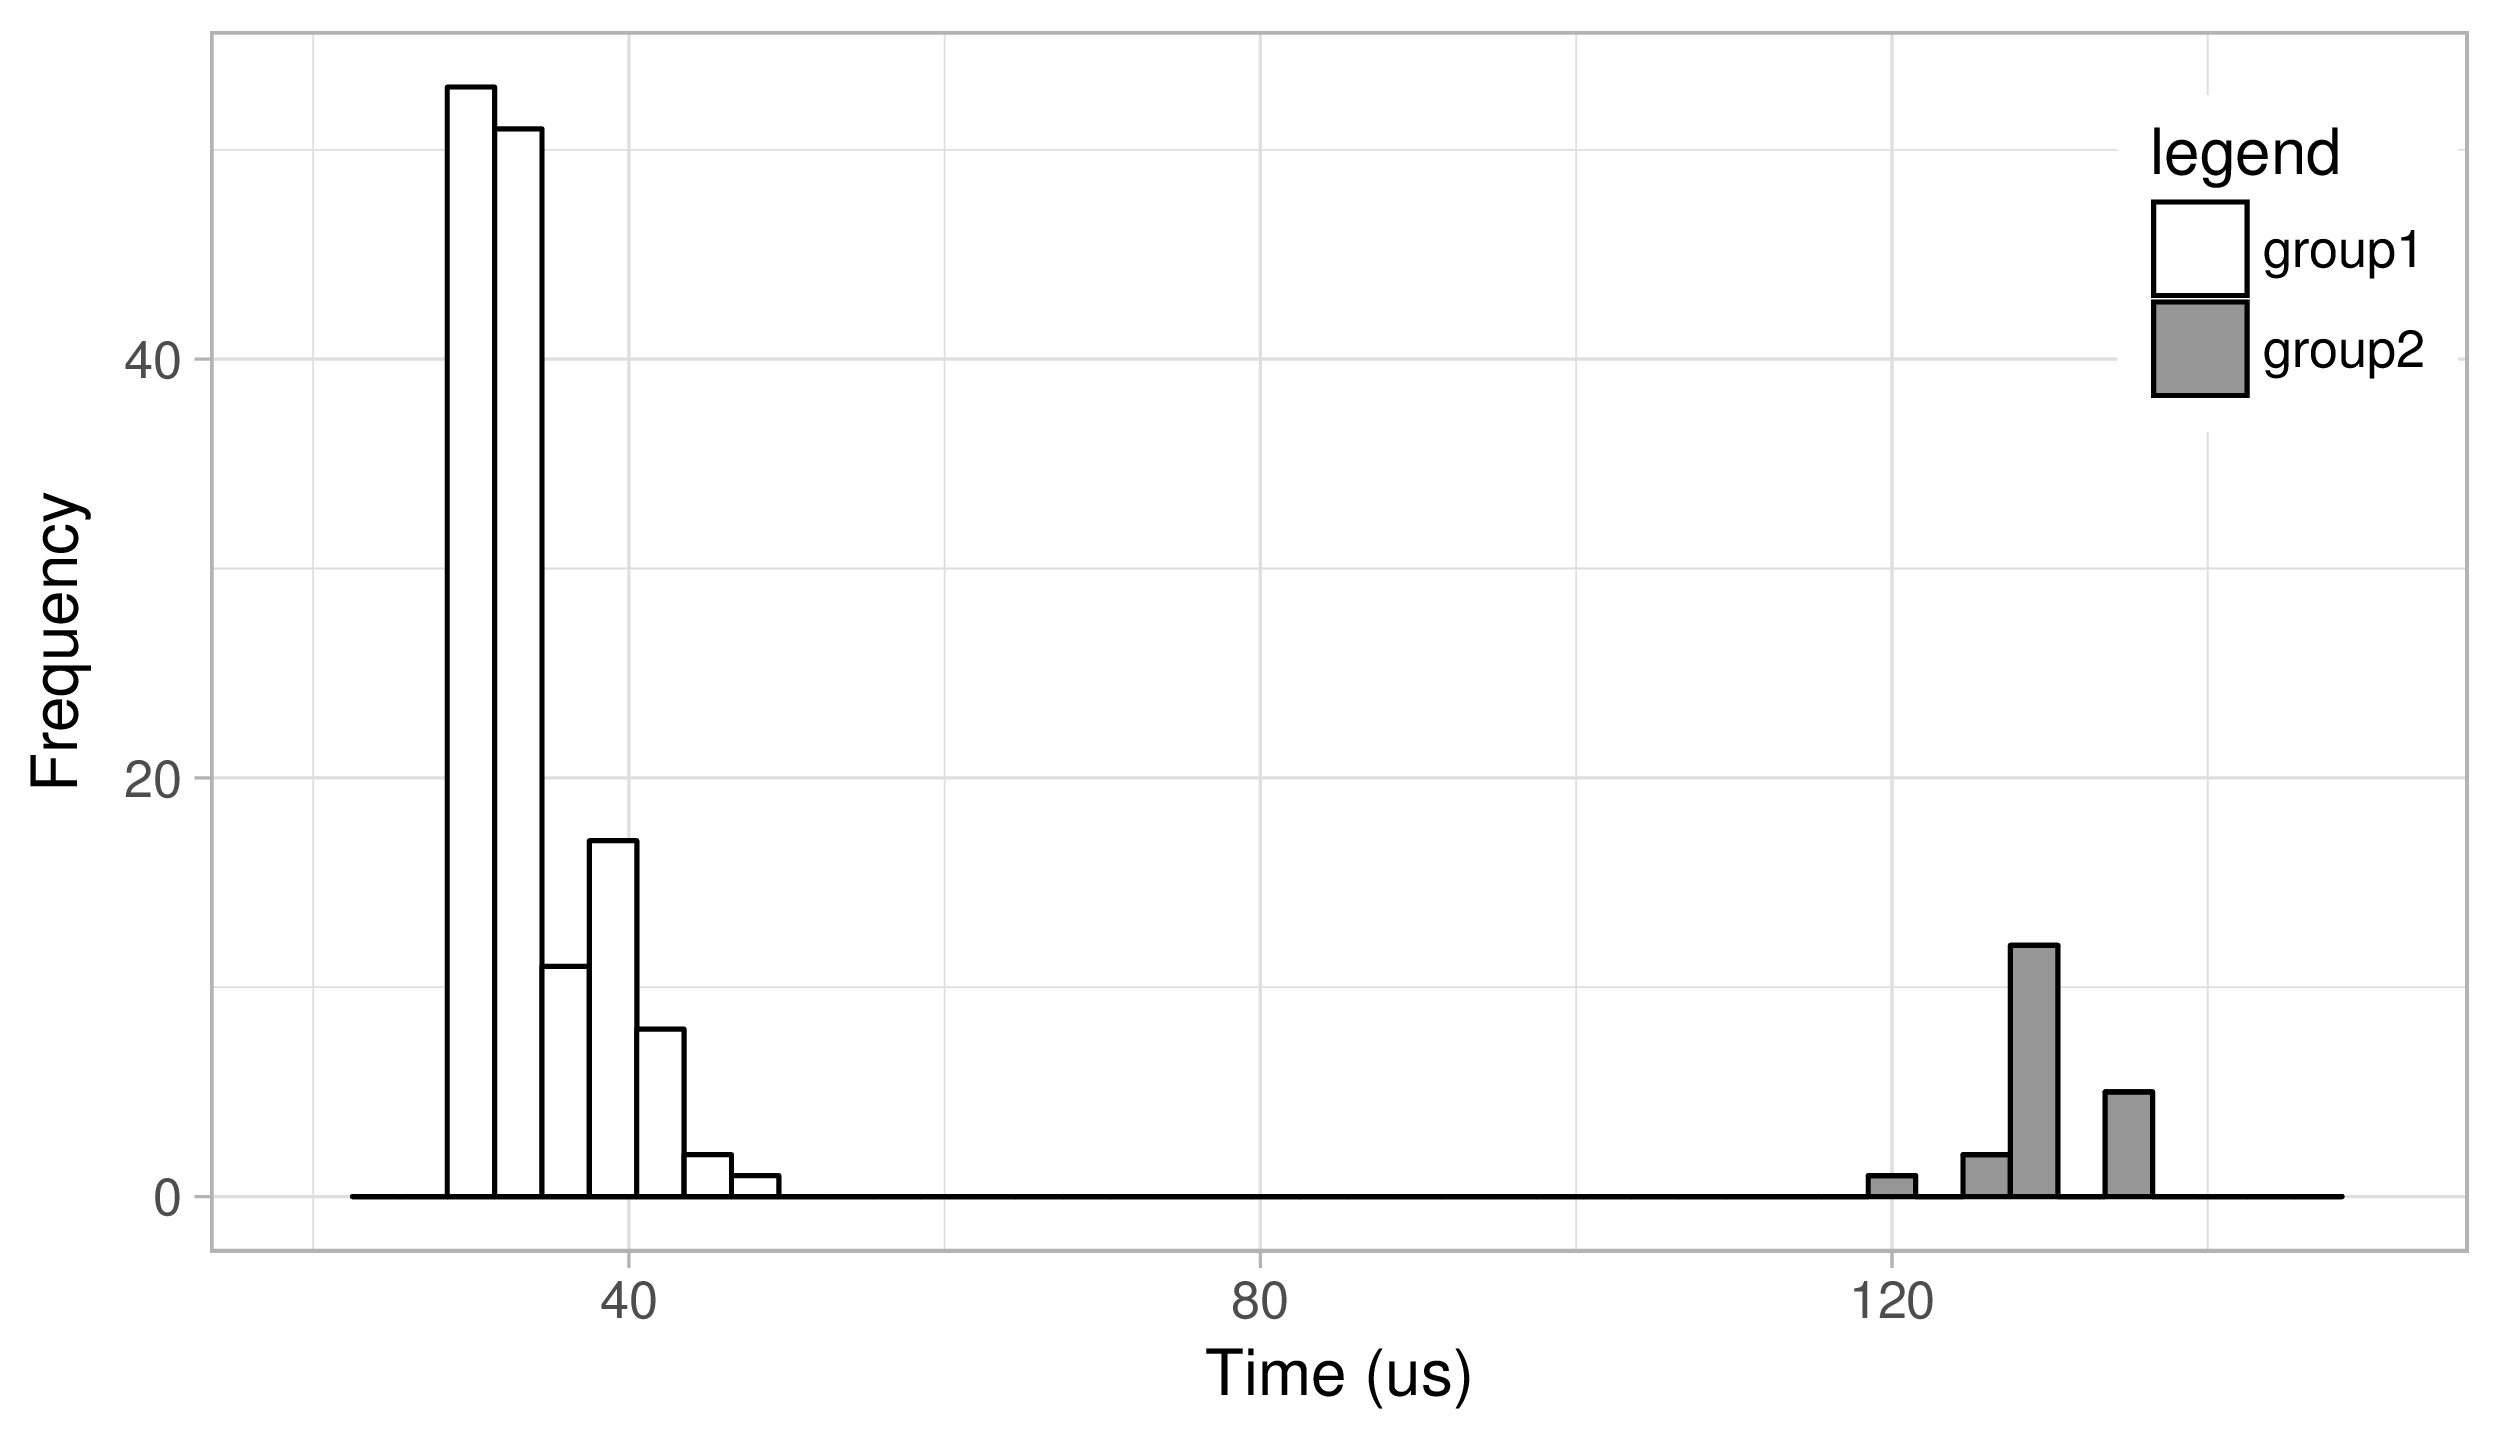
\includegraphics[width=0.50\textwidth]{figures/grouping-hist.png}
        \caption{Automated clustering of the executions into 2 groups}
        \label{fig:grouping-hist}
        \vspace{-10pt}
    \end{figure}

    
\subsection{Association among the Groups}
\label{sec:association}
The clustering of metrics is just a part of the approach, since a rule of groups need to be applied to find the specific cause for the discrepancy on the executions. To solve this problem and find the cause of the difference, after the grouping mechanism we applied a set association rule. Therefore, using a set exclusion, we can find the metric that is responsible for the elapsed time.
The association rule is illustrated on the Figure \ref{fig:association}, which describes a metric X and the elapsed time comparison. The grouping on the Metric x divides the data in two groups and those groups are the intrinsic related to the elapsed time group. \\
The association rule can be applied in an arbitrary classification algorithm with several different dimensions, so the association can be defined as a heuristic to find root cause problems using grouping or clustering algorithms.

A matrix of groups correlation can be done to better understand the relation among the groups.


    % \begin{figure}[h]
    %   \centering
    %     \includegraphics[width=0.50\textwidth]{figures/association.png}
    %     \caption{Association of groups through Apriori algorithm}
    %     \label{fig:association}
    % \end{figure}
    
\begin{table}[h]
\centering
\begin{tabular}{cccc}
                      & A                         & B                        & C     \\ \hline
                      &                           &                          &       \\ 
A                     & X                         & 75\%                     & 100\% \\ \hline
                      &                           &                          &       \\ 
B                     & 75\%                      & X                        & 65\%  \\ \hline
                      &                           &                          &       \\
\multicolumn{1}{l}{C} & \multicolumn{1}{l}{100\%} & \multicolumn{1}{l}{65\%} & X     \\ \hline
\end{tabular}
\vspace{10pt}
\caption{Association of groups through Apriori algorithm}
\label{fig:association}
\end{table}

\subsection{Accuracy of the model}
The association will give the group of metrics that are related with slow and fast runs, however, there is the possibility of false positives and false negatives. The accuracy of the model is related with the size of the groups given, i.e. the all slow executions will be in one group, however the related metric, which explains the reason, is bigger than the associated group.  In summary, if the groups overlap, main metric and slow executions, no false positives of negatives were found, even though the overlap does not mean is responsible for the performance problem, it is only an indication factor. In this matter, statistics is an indicator of underlying causes, which requires some complementary analysis to be confirmed.
